\documentclass[14pt]{beamer}
\usepackage{fontspec}
\usepackage{color}

%% These fonts are non-free.
%% Comment out the lines if you don't have them.
\setmainfont{Equity Text A}
\setsansfont{Concourse T3}
\setmonofont{Triplicate T4}

\definecolor{bgcolor}{RGB}{20,25,28}
\definecolor{codecolor}{RGB}{249,38,114}
\hypersetup{colorlinks,linkcolor=,urlcolor=codecolor}
\setbeamercolor{background canvas}{bg=bgcolor}
\setbeamercolor{normal text}{fg=white}
\setbeamertemplate{navigation symbols}{}

\begin{document}
\begin{frame}
  \begin{center}
    
\includegraphics[width=0.5\columnwidth]{portacle.png}
    \url{https://portacle.github.io}
  \end{center}
\end{frame}

\begin{frame}
  \begin{center}
    
\includegraphics[width=0.5\columnwidth]{components.png}
  \end{center}
\end{frame}

\begin{frame}
  \begin{center}
    
\includegraphics[width=0.5\columnwidth]{systems.png}
  \end{center}
\end{frame}

\begin{frame}
  \begin{center}
    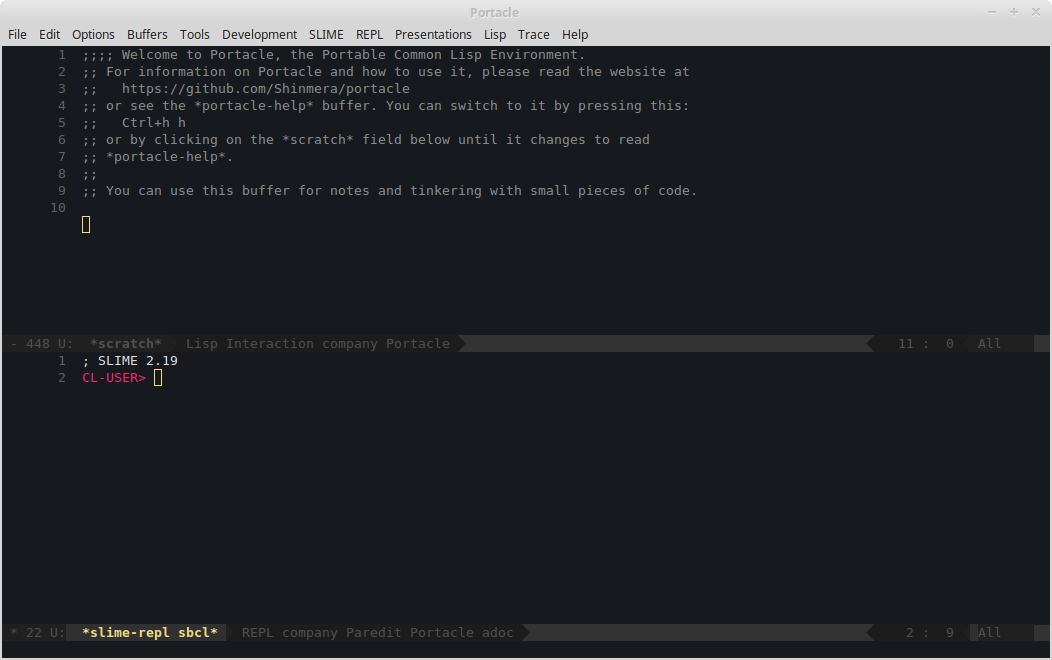
\includegraphics[width=1.0\columnwidth]{portacle-start.png}
  \end{center}
\end{frame}

\begin{frame}
  \begin{center}
    
\includegraphics[width=0.5\columnwidth]{portacle.png}
    \url{https://portacle.github.io}
  \end{center}
\end{frame}

\end{document}

%%% Local Variables:
%%% mode: latex
%%% TeX-master: t
%%% TeX-engine: luatex
%%% End:
